% Chapter 0: Introduction
% Harvard-quality academic presentation
% Bachelor program, Bucharest University of Economic Studies

\documentclass[9pt, aspectratio=169, t]{beamer}

% Ensure content fits on slides
\setbeamersize{text margin left=8mm, text margin right=8mm}

%=============================================================================
% THEME AND STYLE CONFIGURATION
%=============================================================================
\usetheme{default}
% Using default theme for clean header/footer control

% Color Palette (matching Redispatch PDF)
\definecolor{MainBlue}{RGB}{26, 58, 110}
\definecolor{AccentBlue}{RGB}{26, 58, 110}
\definecolor{IDAred}{RGB}{205, 0, 0}
\definecolor{DarkGray}{RGB}{51, 51, 51}
\definecolor{MediumGray}{RGB}{128, 128, 128}
\definecolor{LightGray}{RGB}{248, 248, 248}
\definecolor{VeryLightGray}{RGB}{235, 235, 235}
\definecolor{KeynoteGray}{RGB}{218, 218, 218}
\definecolor{SectionGray}{RGB}{120, 120, 120}
\definecolor{FooterGray}{RGB}{100, 100, 100}
\definecolor{Crimson}{RGB}{220, 53, 69}
\definecolor{Forest}{RGB}{46, 125, 50}
\definecolor{Amber}{RGB}{181, 133, 63}
\definecolor{Orange}{RGB}{230, 126, 34}
\definecolor{Purple}{RGB}{142, 68, 173}

% Gradient background (exact Keynote 315° gradient: white to RGB 218,218,218)
\setbeamertemplate{background}{%
    \begin{tikzpicture}[remember picture, overlay]
        \shade[shading=axis, shading angle=315,
        top color=white, bottom color=KeynoteGray]
        (current page.south west) rectangle (current page.north east);
    \end{tikzpicture}%
}
% Fallback solid color for compatibility
\setbeamercolor{background canvas}{bg=}

\setbeamercolor{palette primary}{bg=MainBlue, fg=white}
\setbeamercolor{palette secondary}{bg=MainBlue!85, fg=white}
\setbeamercolor{palette tertiary}{bg=MainBlue!70, fg=white}
\setbeamercolor{structure}{fg=MainBlue}
\setbeamercolor{title}{fg=IDAred}
\setbeamercolor{frametitle}{fg=IDAred, bg=}
\setbeamercolor{block title}{bg=MainBlue, fg=white}
\setbeamercolor{block body}{bg=VeryLightGray, fg=DarkGray}
\setbeamercolor{block title alerted}{bg=Crimson, fg=white}
\setbeamercolor{block body alerted}{bg=Crimson!8, fg=DarkGray}
\setbeamercolor{block title example}{bg=Forest, fg=white}
\setbeamercolor{block body example}{bg=Forest!8, fg=DarkGray}
\setbeamercolor{item}{fg=MainBlue}

% Footer colors (override Madrid theme blue)
\setbeamercolor{author in head/foot}{fg=FooterGray, bg=}
\setbeamercolor{title in head/foot}{fg=FooterGray, bg=}
\setbeamercolor{date in head/foot}{fg=FooterGray, bg=}
\setbeamercolor{section in head/foot}{fg=FooterGray, bg=}
\setbeamercolor{subsection in head/foot}{fg=FooterGray, bg=}

% Bullet styles (apply everywhere including blocks)
\setbeamertemplate{itemize item}{\color{MainBlue}$\boxdot$}
\setbeamertemplate{itemize subitem}{\color{MainBlue}$\blacktriangleright$}
\setbeamertemplate{itemize subsubitem}{\color{MainBlue}\tiny$\bullet$}
\setbeamertemplate{itemize/enumerate body begin}{\normalsize}
\setbeamertemplate{itemize/enumerate subbody begin}{\normalsize}

% Item spacing - compact style
\setlength{\leftmargini}{10pt}       % Level 1: minimal indent
\setlength{\leftmarginii}{10pt}      % Level 2: minimal additional indent
% Compact list spacing (zero extra space before/after lists in blocks)
\makeatletter
\def\@listi{\leftmargin\leftmargini \topsep 0pt \parsep 0pt \itemsep 0pt}
\def\@listii{\leftmargin\leftmarginii \topsep 0pt \parsep 0pt \itemsep 0pt}
\makeatother

\setbeamertemplate{navigation symbols}{}

%=============================================================================
% CUSTOM HEADLINE
%=============================================================================
\setbeamertemplate{headline}{%
    \vskip10pt%
    \hbox to \paperwidth{%
        \hskip0.5cm%
        {\small\color{FooterGray}\renewcommand{\hyperlink}[2]{##2}\insertsectionhead}%
        \hfill%
        \textcolor{FooterGray}{\small\insertframenumber}%
        \hskip0.5cm%
    }%
    \vskip4pt%
    {\color{FooterGray}\hrule height 0.4pt}%
}

%=============================================================================
% CUSTOM FOOTER
%=============================================================================
\usepackage{fontawesome5}

\setbeamertemplate{footline}{%
    {\color{FooterGray}\hrule height 0.4pt}%
    \vskip4pt%
    \hbox to \paperwidth{%
        \hskip0.5cm%
        \textcolor{FooterGray}{\small Statistics of Financial Markets}%
        \hfill%
        \raisebox{-0.1em}{%
            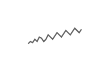
\begin{tikzpicture}[x=0.08em, y=0.08em, line width=0.4pt]
                \draw[FooterGray] (0,3) -- (1,4) -- (2,3.5) -- (3,5) -- (4,4) -- (5,6) -- (6,5.5) -- (7,4) -- (8,5) -- (9,7) -- (10,6) -- (11,5) -- (12,6.5) -- (13,8) -- (14,7) -- (15,6) -- (16,7.5) -- (17,9) -- (18,8) -- (19,7) -- (20,8.5) -- (21,10) -- (22,9) -- (23,8) -- (24,9.5);
            \end{tikzpicture}%
        }%
        \hskip0.5cm%
    }%
    \vskip6pt%
}

%=============================================================================
% PACKAGES
%=============================================================================
\usepackage[utf8]{inputenc}
\usepackage[T1]{fontenc}
\usepackage{amsmath, amssymb, amsthm}
\usepackage{mathtools}
\usepackage{bm}
\usepackage{tikz}
\usetikzlibrary{arrows.meta, positioning, shapes, calc, decorations.pathreplacing, shadings}
\usepackage{booktabs}
\usepackage{multirow}
\usepackage{array}
\usepackage{graphicx}
\usepackage{hyperref}
\usepackage{colortbl}
\usepackage{listings}
\lstset{language=Python, basicstyle=\ttfamily\scriptsize, keywordstyle=\color{MainBlue}\bfseries,
  commentstyle=\color{Forest}, stringstyle=\color{Crimson}, breaklines=true,
  frame=none, backgroundcolor=\color{VeryLightGray}, xleftmargin=2mm}
\hypersetup{colorlinks=true, linkcolor=MainBlue, urlcolor=MainBlue}
\graphicspath{{../../logos/}{../../charts/}{../../photos/}}
\hfuzz=2pt  % Suppress tiny overfull warnings (<2pt)
\vfuzz=2pt  % Suppress tiny vertical overfull warnings (<2pt)

%=============================================================================
% QUANTLET COMMAND
%=============================================================================
\newcommand{\quantlet}[2]{%
    \hfill\href{#2}{%
        \raisebox{-0.15em}{
\includegraphics[height=0.7em]{ql_logo.png}}%
        \textcolor{MainBlue}{\tiny\ #1}%
    }%
}

%=============================================================================
% CUSTOM TITLE PAGE
%=============================================================================
\defbeamertemplate*{title page}{hybrid}[1][]
{
    \vspace{0.2cm}
    % Logos row - top header (with clickable links)
    \begin{center}
        \href{https://www.ase.ro}{
\includegraphics[height=1.0cm]{ase_logo.png}}\hspace{0.3cm}%
        \href{https://theida.net}{
\includegraphics[height=1.0cm]{ida_logo.png}}\hspace{0.3cm}%
        \href{https://blockchain-research-center.com}{
\includegraphics[height=1.0cm]{brc_logo.png}}\hspace{0.3cm}%
        \href{https://www.ai4efin.ase.ro}{
\includegraphics[height=1.0cm]{ai4efin_logo.png}}\hspace{0.3cm}%
        \href{https://ipe.ro/new}{
\includegraphics[height=1.0cm]{acad_logo.png}}\hspace{0.3cm}%
        \href{https://www.digital-finance-msca.com}{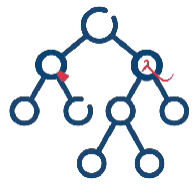
\includegraphics[height=1.0cm]{msca_logo.png}}%
    \end{center}

    \vspace{0.6cm}

    % Main title with Q logos on sides (with clickable links)
    \begin{center}
        \begin{minipage}{0.1\textwidth}
            \centering
            \href{https://quantlet.com}{
\includegraphics[height=1.1cm]{ql_logo.png}}
        \end{minipage}%
        \begin{minipage}{0.78\textwidth}
            \centering
            {\LARGE\bfseries\usebeamercolor[fg]{title}\inserttitle}

            \vspace{0.3cm}

            {\usebeamerfont{subtitle}\usebeamercolor[fg]{title}\insertsubtitle}
        \end{minipage}%
        \begin{minipage}{0.1\textwidth}
            \centering
            \href{https://quantinar.com}{
\includegraphics[height=1.1cm]{qr_logo.png}}
        \end{minipage}
    \end{center}

    \vspace{0.6cm}

    % Authors (left aligned)
    \hspace{0.5cm}{\usebeamerfont{author}\insertauthor}

    \vspace{0.3cm}

    % Institute/Affiliations (left aligned)
    \hspace{0.5cm}\begin{minipage}[t]{0.9\textwidth}
        \raggedright\small\insertinstitute
    \end{minipage}
}

%=============================================================================
% THEOREM ENVIRONMENTS
%=============================================================================
\theoremstyle{definition}
\setbeamertemplate{theorems}[numbered]
\newtheorem{defn}{Definition}
\newtheorem{thm}{Theorem}
\newtheorem{prop}{Proposition}
\newtheorem{rmk}{Remark}

%=============================================================================
% CENTRED MINIPAGE (no extra vertical space)
%=============================================================================
\newenvironment{cminipage}[1]{%
    \par\noindent\hfill\begin{minipage}{#1}\ignorespaces
}{%
    \end{minipage}\hfill\null\par
}

%=============================================================================
% CUSTOM COMMANDS
%=============================================================================
\newcommand{\E}{\mathbb{E}}
\newcommand{\Var}{\text{Var}}
\newcommand{\Cov}{\text{Cov}}
\newcommand{\Corr}{\text{Corr}}
\newcommand{\R}{\mathbb{R}}
\newcommand{\N}{\mathbb{N}}
\newcommand{\Z}{\mathbb{Z}}
\newcommand{\B}{\mathbf{B}}
\newcommand{\imark}{\textcolor{MainBlue}{\textbullet}}
\newcommand{\RMSE}{\text{RMSE}}
\newcommand{\MAE}{\text{MAE}}
\newcommand{\MAPE}{\text{MAPE}}

%=============================================================================
% TITLE INFORMATION
%=============================================================================
\title[Statistics of Financial Markets]{Statistics of Financial Markets}
\subtitle{Chapter 0: Introduction}
\author[D.T. Pele]{Daniel Traian PELE}
\institute{Bucharest University of Economic Studies\\
IDA Institute Digital Assets\\
Blockchain Research Center\\
AI4EFin Artificial Intelligence for Energy Finance\\
Romanian Academy, Institute for Economic Forecasting\\
MSCA Digital Finance}
\date{}

%=============================================================================
% BEGIN DOCUMENT
%=============================================================================
\begin{document}

%=============================================================================
% TITLE SLIDE
%=============================================================================
{
\setbeamertemplate{headline}{}
\setbeamertemplate{footline}{}
\begin{frame}[noframenumbering]
    \titlepage
\end{frame}
}

%#############################################################################
% SECTION: Motivation
%#############################################################################
\section{Motivation}

%-----------------------------------------------------------------------------
% Slide: It's the financial market!
%-----------------------------------------------------------------------------
\begin{frame}{It's the financial market!}
    \begin{center}
        % Image: Clinton meme -- "It's the economy, Stupid!" adapted to "It's the financial market!"
        % \includegraphics[width=0.55\textwidth]{clinton_meme.png}
        \vspace{2cm}
        {\Large\color{MediumGray}\textit{[Image placeholder: Clinton meme -- ``It's the economy, Stupid!'']}}
    \end{center}
\end{frame}

%-----------------------------------------------------------------------------
% Slide: Why Study Statistics of Financial Markets (SFM)?
%-----------------------------------------------------------------------------
\begin{frame}{Why Study Statistics of Financial Markets (SFM)?}
    \begin{itemize}
        \item Financial markets are highly complex, dynamic, and volatile.
        \item Risk and return trade-offs must be carefully analyzed to make informed investment decisions.
        \item Pricing, hedging, and portfolio management depend on quantitative and statistical models.
        \item Data-driven decision-making is fundamental in finance, especially with the rise of big data and machine learning.
        \item Modern finance relies heavily on statistical techniques for
        \begin{itemize}
            \item Asset pricing models (CAPM, APT)
            \item Risk management (VaR, Expected Shortfall)
            \item Portfolio optimization (Mean-Variance Analysis, Black-Litterman)
            \item Algorithmic trading and market microstructure analysis
        \end{itemize}
    \end{itemize}
\end{frame}

%-----------------------------------------------------------------------------
% Slide: Real-World Applications of SFM (1/2)
%-----------------------------------------------------------------------------
\begin{frame}{Real-World Applications of SFM}
    \begin{itemize}
        \item Asset Pricing \& Return Prediction
        \begin{itemize}
            \item Determine the fair price of financial assets using statistical models.
            \item Capital Asset Pricing Model (CAPM), Fama-French multifactor models.
            \item Machine learning-based return prediction models.
            \item Statistical arbitrage and factor-based investing.
        \end{itemize}
        \item Risk Management \& Financial Stability
        \begin{itemize}
            \item Quantify financial risk, measure volatility, and manage portfolio risk.
            \item Value at Risk (VaR) \& Conditional Value at Risk (CVaR).
            \item Risk-neutral pricing and Monte Carlo simulations.
            \item Extreme Value Theory (EVT) for tail risk estimation.
            \item Stress testing and scenario analysis for regulatory compliance (Basel III, Solvency II).
        \end{itemize}
    \end{itemize}
\end{frame}

%-----------------------------------------------------------------------------
% Slide: Real-World Applications of SFM (2/2)
%-----------------------------------------------------------------------------
\begin{frame}{Real-World Applications of SFM}
    \begin{itemize}
        \item Algorithmic \& High-Frequency Trading
        \begin{itemize}
            \item Goal: Use quantitative models to develop profitable trading strategies.
            \item Statistical arbitrage using co-integration models.
            \item Market impact modeling and execution strategies.
            \item Market-making and liquidity provision models.
            \item High-frequency trading using machine learning (LSTMs, deep reinforcement learning).
        \end{itemize}
        \item Credit Risk \& Financial Stability
        \begin{itemize}
            \item Goal: Assess the probability of default and financial system stability.
            \item Credit scoring models (e.g., Logistic Regression, Random Forests).
            \item Structural models of credit risk (Merton Model).
            \item Reduced-form models (Jarrow-Turnbull model).
            \item Systemic risk indicators and contagion modeling.
        \end{itemize}
    \end{itemize}
\end{frame}

%-----------------------------------------------------------------------------
% Slide: How Statistics Helps in Financial Markets
%-----------------------------------------------------------------------------
\begin{frame}{How Statistics Helps in Financial Markets}
    \begin{itemize}
        \item Detecting Market Trends and Anomalies
        \begin{itemize}
            \item Identifying arbitrage opportunities, mean reversion patterns, and seasonal trends.
        \end{itemize}
        \item Building Predictive Models for Asset Prices
        \begin{itemize}
            \item Applying machine learning, time series analysis, and econometric methods.
        \end{itemize}
        \item Measuring and Managing Financial Risk
        \begin{itemize}
            \item Using statistical risk metrics, stress testing, and scenario analysis.
        \end{itemize}
        \item Validating Financial Theories with Empirical Data
        \begin{itemize}
            \item Efficient Market Hypothesis (EMH)
            \item Behavioral Finance theories
            \item Asset Pricing Models
        \end{itemize}
    \end{itemize}
\end{frame}

%-----------------------------------------------------------------------------
% Slide: Rise of the machines (1/2) -- Cray 2
%-----------------------------------------------------------------------------
\begin{frame}{Rise of the machines}
    \begin{columns}[T]
        \begin{column}{0.48\textwidth}
            \begin{itemize}
                \item \underline{Cray 2}: world's fastest supercomputer: 1985--1990
                \item 1.9 GFLOPs
                \item 5,500 pounds
                \item \$49,863,243.49 million (current \$)
                \item $10^{\wedge}$(G=9, T=12, P=15, E=18)
            \end{itemize}
            \vspace{0.5cm}
            {\small\color{IDAred} G = Giga, T = Tera, P = Peta, E = Exa}
        \end{column}
        \begin{column}{0.48\textwidth}
            % Image: Cray 2 supercomputer photo
            % \includegraphics[width=\textwidth]{cray2.png}
            \begin{center}
                {\Large\color{MediumGray}\textit{[Image: Cray 2 supercomputer]}}
            \end{center}
        \end{column}
    \end{columns}
\end{frame}

%-----------------------------------------------------------------------------
% Slide: Rise of the machines (2/2) -- iPhone
%-----------------------------------------------------------------------------
\begin{frame}{Rise of the machines}
    \begin{columns}[T]
        \begin{column}{0.48\textwidth}
            \begin{itemize}
                \item 2016 iPhone 7, 178 GFLOPs
                \item 2021 iPhone 13, 1200 GFLOPs
                \item 2025 iPhone 16, 2.15 TFLOPS
                \item 170 g = 1K EUR
                \item $10^{\wedge}$(G9, T12, P15, E18)
            \end{itemize}
        \end{column}
        \begin{column}{0.48\textwidth}
            % Image: iPhone, A18 chip, Cray 2 board comparison
            % \includegraphics[width=\textwidth]{iphone_vs_cray.png}
            \begin{center}
                {\Large\color{MediumGray}\textit{[Image: A18 chip, Cray board, iPhone]}}
            \end{center}
        \end{column}
    \end{columns}
\end{frame}

%-----------------------------------------------------------------------------
% Slide: Cryptocurrency Milestones
%-----------------------------------------------------------------------------
\begin{frame}{Cryptocurrency Milestones}
    % Image: S&P Cryptocurrency MegaCap Index chart with animated overlays
    % In the PDF this is presented as progressive chart builds showing key events.
    % Here we summarize all milestones on a single slide.

    \begin{center}
        % \includegraphics[width=0.85\textwidth]{sp_crypto_megacap_index.png}
        {\Large\color{MediumGray}\textit{[Chart: S\&P Cryptocurrency MegaCap Index, 2017--2025]}}
    \end{center}

    \vspace{0.2cm}

    \begin{columns}[T]
        \begin{column}{0.48\textwidth}
            \begin{itemize}\small
                \item 2017 Boom \& 2018 Bubble Crash
                \item 2020 May -- Bitcoin 3rd Halving
                \item 2020 Boom \& 2021 Bubble Crash
                \item 2021 NFT Boom
                \item 2022 Apr -- SEC Regulation
            \end{itemize}
        \end{column}
        \begin{column}{0.48\textwidth}
            \begin{itemize}\small
                \item 2022 Nov -- FTX Belly Up
                \item 2024 Jan -- BTC Spot ETF
                \item 2024 Apr -- BTC 4th Halving
                \item 2024 May -- ETH Spot ETF
                \item 2024 Nov -- Trump Elected
            \end{itemize}
        \end{column}
    \end{columns}

    \vspace{0.2cm}
    {\footnotesize\textit{Data Source: S\&P Cryptocurrency MegaCap Index -- Jan 14, 2025.}}
\end{frame}

%-----------------------------------------------------------------------------
% Slide: Speculative Bubbles
%-----------------------------------------------------------------------------
\begin{frame}{Speculative Bubbles}
    \begin{columns}[T]
        \begin{column}{0.58\textwidth}
            \small
            Back in the spring of 1720, Sir Isaac Newton owned shares in the South Sea Company, the hottest stock in England. As a rumor among the people appeared that ore of silver/gold was found, this was ``fake news'' as we call them today. The great physicist muttered that he \textcolor{IDAred}{`could calculate the motions of the heavenly bodies, but not the madness of the people.'} Newton dumped his South Sea shares, pocketing a 100\% profit totaling \pounds 7,000. But just months later, swept up in the wild enthusiasm of the market, Newton jumped back in at a much higher price --- and lost \pounds 20,000 (or more than \pounds 5 million in 2025's money.) For the rest of his life, he forbade anyone to speak the words `South Sea' in his presence.

            \vspace{0.3cm}

            % Image: South Sea Stock chart December 1718 - December 1721
            % \includegraphics[width=\textwidth]{south_sea_stock.png}
            {\color{MediumGray}\textit{[Chart: South Sea Stock, Dec 1718 -- Dec 1721]}}
        \end{column}
        \begin{column}{0.38\textwidth}
            % Image: Isaac Newton portrait
            % \includegraphics[width=0.9\textwidth]{newton_portrait.png}
            \begin{center}
                {\color{MediumGray}\textit{[Image: Newton portrait]}}
            \end{center}

            \vspace{0.5cm}

            % Image: Tree with apples illustration
            % \includegraphics[width=0.7\textwidth]{newton_tree.png}
            \begin{center}
                {\color{MediumGray}\textit{[Image: Newton's apple tree]}}
            \end{center}

            \vspace{0.3cm}
            \href{https://doi.org/10.2139/ssrn.3389182}{\underline{Andrew Odlyzko (2019)}}
        \end{column}
    \end{columns}
\end{frame}

%-----------------------------------------------------------------------------
% Slide: Intrinsic values of CC
%-----------------------------------------------------------------------------
\begin{frame}{Intrinsic values of CC}
    \begin{columns}[T]
        \begin{column}{0.45\textwidth}
            \begin{itemize}
                \item Eventually zero or further adoption?
                \item Metcalfe's law: $p$ market cap,
                \begin{itemize}
                    \item $p = e^{\alpha_0} u^{\beta_0}$ and $\beta_0 = 2$.
                    \item $u$: \# active users, i.e.\ addresses
                \end{itemize}
                \item (Generalized) Metcalfe's law:
                \[
                    \log(p) = \alpha + \beta \log(u) + \varepsilon
                \]
            \end{itemize}

            \vspace{0.5cm}
            \href{https://doi.org/10.1016/j.econlet.2018.09.013}{\underline{Wheatley S et al (2018)}}
        \end{column}
        \begin{column}{0.52\textwidth}
            % Image: Log-log plot of Market Cap (USD) vs Active Users, with Metcalfe fit line
            % \includegraphics[width=\textwidth]{metcalfe_law_btc.png}
            \begin{center}
                {\color{MediumGray}\textit{[Chart: Market Cap vs Active Users, log-log scale]}}
            \end{center}

            \vspace{1cm}

            \hfill\href{https://quantinar.com}{
\includegraphics[height=0.8cm]{qr_logo.png}}
            \textcolor{MainBlue}{CC returns}
        \end{column}
    \end{columns}
\end{frame}

%-----------------------------------------------------------------------------
% Slide: Bubbles
%-----------------------------------------------------------------------------
\begin{frame}{Bubbles}
    \begin{columns}[T]
        \begin{column}{0.45\textwidth}
            \begin{itemize}
                \item Market-to-Metcalfe value ratio
            \end{itemize}
            \[
                \text{MMV}_i = \frac{p_i}{e^{\alpha} u_i^{\beta}}
            \]

            after log-log regression fit,
            \[
                (\alpha, \beta) = (-1.75,\; 2.12)
            \]

            \begin{itemize}
                \item Six bubbles identified
            \end{itemize}

            \vspace{0.5cm}
            \href{https://doi.org/10.1016/j.econlet.2018.09.013}{\underline{Wheatley S et al (2018)}}
        \end{column}
        \begin{column}{0.52\textwidth}
            % Image: MMV ratio time series chart 2010-2024 with colored bubble periods
            % \includegraphics[width=\textwidth]{mmv_bubbles.png}
            \begin{center}
                {\color{MediumGray}\textit{[Chart: MMV ratio, 2010--2024, six bubbles highlighted]}}
            \end{center}

            \vspace{1cm}

            \hfill\href{https://quantinar.com}{
\includegraphics[height=0.8cm]{qr_logo.png}}
            \textcolor{MainBlue}{CC returns}
        \end{column}
    \end{columns}
\end{frame}

%-----------------------------------------------------------------------------
% Slide: The New Gold
%-----------------------------------------------------------------------------
\begin{frame}{The New Gold}
    \begin{columns}[T]
        \begin{column}{0.62\textwidth}
            \begin{itemize}
                \item Market Cap Gold (Apr 27, 2023) \hfill 13,192 Billion USD
                \item Market Cap BTC (Apr 27, 2023) \hfill 559 Billion USD
            \end{itemize}
            \hfill $\Big\}$ 4.2\,\%

            \vspace{0.5cm}

            \begin{itemize}
                \item Market Cap Gold (Jan 16, 2025) \hfill 18.318 Trillion USD
                \item Market Cap BTC (Jan 16, 2025) \hfill 1.972 Trillion USD
            \end{itemize}
            \hfill $\Big\}$ 9.29\,\%

            \vspace{0.8cm}

            If BTC, CCs are seen as store of value then price can still grow a lot.

            \vspace{0.3cm}
            \href{https://companiesmarketcap.com/bitcoin/marketcap/}{\underline{Bitcoin's Market Capitalization History}}
        \end{column}
        \begin{column}{0.35\textwidth}
            % Image: Gold coin with BTC overlay
            % \includegraphics[width=0.9\textwidth]{gold_btc.png}
            \begin{center}
                {\color{MediumGray}\textit{[Image: Gold coin / BTC]}}
            \end{center}
        \end{column}
    \end{columns}
\end{frame}

%-----------------------------------------------------------------------------
% Slide: The Stochastic Volatility with Correlated Jumps Model
%-----------------------------------------------------------------------------
\begin{frame}{The Stochastic Volatility with Correlated Jumps Model}
    \begin{columns}[T]
        \begin{column}{0.55\textwidth}
            \begin{align*}
                \frac{dS_t}{S_t} &= r\,dt + \sqrt{V_t}\,dW_t^s + Z_t^y\,dN_t \\[6pt]
                dV_t &= \kappa(\theta - V_t)\,dt + \sigma_v\sqrt{V_t}\,dW_t^v + Z_t^v\,dN_t
            \end{align*}
            \[
                \Cov(dW_t^s, dW_t^v) = \rho\,dt, \quad P(dN_t = 1) = \lambda\,dt
            \]
            \[
                Z_t^v \sim \text{Exp}(\mu_v), \quad Z_t^y \mid Z_t^v \sim N(\mu_y + \rho_j Z_t^v,\; \sigma_y^2)
            \]

            \vspace{0.3cm}

            % Image: In-sample and Out-of-sample RMSE box plots and time series for BS, SV, SVJ, SVCJ
            % \includegraphics[width=\textwidth]{svcj_rmse.png}
            {\small\color{MediumGray}\textit{[Charts: RMSE comparison -- BS, SV, SVJ, SVCJ]}}
        \end{column}
        \begin{column}{0.42\textwidth}
            {\footnotesize
            \begin{tabular}{l c c c c}
                \toprule
                & BS & SV & SVJ & SVCJ \\
                \midrule
                $\sigma$ & 0.0278 & & & \\
                $\rho$ & & 0.1462 & $-0.3310$ & $-0.6245$ \\
                $\kappa$ & & 0.2203 & 1.5459 & 0.7425 \\
                $\theta$ & & 0.0006 & 0.0008 & 0.0008 \\
                $V_0$ & & 0.0013 & 0.0009 & 0.0009 \\
                $\sigma_v$ & & 0.0216 & 0.0368 & 0.0489 \\
                $\lambda$ & & & 0.0040 & 0.0033 \\
                $\mu_v$ & & & 0.2359 & 0.3166 \\
                $\rho_j$ & & & & $-1.0821$ \\
                $\sigma_y$ & & & 0.1890 & 0.1267 \\
                $\mu_v$ & & & & 0.0206 \\
                \bottomrule
            \end{tabular}
            }

            \vspace{0.3cm}
            {\footnotesize \href{https://doi.org/10.1007/s11147-022-09188-8}{Teng and Haerdle (2022) Financial analytics of inverse BTC options in a stochastic volatility world}}
        \end{column}
    \end{columns}
\end{frame}

%#############################################################################
% SECTION: Course overview
%#############################################################################
\section{Course overview}

%-----------------------------------------------------------------------------
% Slide: Outline
%-----------------------------------------------------------------------------
\begin{frame}{Outline}
    \begin{enumerate}
        \item Motivation \checkmark
        \item Course overview
        \item Resources
        \item Grading
        \item References
    \end{enumerate}
\end{frame}

%-----------------------------------------------------------------------------
% Slide: Course Objectives
%-----------------------------------------------------------------------------
\begin{frame}{Course Objectives}
    \begin{itemize}
        \item Understand fundamental statistical methods applied in finance.
        \item Develop expertise in probability theory and its applications in financial markets.
        \item Learn time series models (ARIMA, GARCH) for financial data analysis.
        \item Study the Efficient Market Hypothesis (EMH) and its empirical validation.
        \item Explore the Fractal Market Hypothesis (FMH) and long-memory processes.
        \item Understand volatility clustering and its implications for risk modeling.
        \item Analyze risk indicators such as VaR, CVaR, and systemic risk measures.
        \item Learn about credit risk models and their role in financial stability.
        \item Work with real-world financial datasets and Python/R for implementation.
    \end{itemize}
\end{frame}

%-----------------------------------------------------------------------------
% Slide: Key Topics Covered
%-----------------------------------------------------------------------------
\begin{frame}{Key Topics Covered}
    \begin{itemize}\small
        \item Probability \& Statistical Methods in Finance
        \begin{itemize}\small
            \item Probability distributions of asset returns (Normal, Log-normal, t-distribution, Stable distributions).
            \item Monte Carlo simulations for pricing and risk assessment.
            \item Stochastic processes in finance (Brownian motion, L\'{e}vy processes, Fractional Brownian Motion).
        \end{itemize}
        \item Time Series Analysis \& Forecasting
        \begin{itemize}\small
            \item Autoregressive models (AR, ARMA, ARIMA) for return prediction.
            \item Volatility modeling: GARCH, EGARCH, TGARCH.
            \item Volatility clustering: Why volatility is persistent and clustered in financial markets.
        \end{itemize}
        \item Efficient Market Hypothesis (EMH) \& Fractal Market Hypothesis (FMH)
        \begin{itemize}\small
            \item EMH: Weak-form, semi-strong, and strong-form efficiency.
            \item Empirical tests of EMH using statistical techniques (random walk, autocorrelation, variance ratio tests).
            \item FMH: Non-stationary behavior of financial markets, self-similarity, and long-memory processes.
        \end{itemize}
        \item Volatility Clustering \& Financial Stability
        \begin{itemize}\small
            \item Volatility Clustering: Why financial markets exhibit persistent periods of high/low volatility.
            \item Leverage Effect: How negative shocks increase volatility more than positive shocks.
            \item Risk Indicators: Value at Risk (VaR), Conditional VaR (CVaR).
        \end{itemize}
        \item Credit Risk \& Default Prediction
        \begin{itemize}\small
            \item Credit scoring models
            \item Stress testing and Basel III regulatory framework.
        \end{itemize}
    \end{itemize}
\end{frame}

%#############################################################################
% SECTION: Resources
%#############################################################################
\section{Resources}

%-----------------------------------------------------------------------------
% Slide: Resources
%-----------------------------------------------------------------------------
\begin{frame}{Resources}
    \begin{thebibliography}{99}
        \bibitem{FHH2019} Franke, J., H\"{a}rdle, W.K., Hafner, C.M. (2019).
        \textit{Statistics of Financial Markets: An Introduction}. 4th ed., Springer.

        \bibitem{Roman2003} Roman, M. (2003).
        \textit{Statistica financiar-bancara}. ASE Bucharest.

        \bibitem{CLM1997} Campbell, J.Y., Lo, A.W., MacKinlay, A.C. (1997).
        \textit{The Econometrics of Financial Markets}. Princeton University Press.

        \bibitem{Hand2010} Hand, D.J. (2010).
        \textit{Statistics in Finance}. In: International Encyclopedia of Statistical Science, Springer.

        \bibitem{Pele2013} Pele, D.T. (2013).
        \textit{Criza pie\c{t}elor de capital. O abordare interdisciplinar\u{a}}. ASE Bucharest.

        \bibitem{Tsay2010} Tsay, R.S. (2010).
        \textit{Analysis of Financial Time Series}. 3rd ed., Wiley.

        \bibitem{Quantinar} Quantinar -- \url{https://quantinar.com}
    \end{thebibliography}
\end{frame}

%#############################################################################
% SECTION: Grading
%#############################################################################
\section{Grading}

%-----------------------------------------------------------------------------
% Slide: Grading
%-----------------------------------------------------------------------------
\begin{frame}{Grading}
    \vspace{1cm}
    \begin{center}
        \begin{block}{Final Grade}
            \centering\large
            \[
                \text{Final Grade} = 0.7 \times \text{Exam} + \text{Seminar}
            \]
        \end{block}

        \vspace{0.8cm}

        \begin{block}{Seminar Grade}
            \centering\large
            \[
                \text{Seminar} = 0.2 \times \text{Project} + 0.1 \times \text{Attendance}
            \]
        \end{block}
    \end{center}
\end{frame}

%#############################################################################
% SECTION: References
%#############################################################################
\section{References}

%-----------------------------------------------------------------------------
% Slide: References
%-----------------------------------------------------------------------------
\begin{frame}{References}
    \begin{thebibliography}{99}
        \bibitem{Wheatley2018} Wheatley, S., Sornette, D., Huber, T., Reppen, M., Gantner, R.N. (2018).
        Are Bitcoin bubbles predictable? Combining a generalized Metcalfe's Law and the Log-Periodic Power Law Singularity model.
        \textit{Royal Society Open Science}, 6(6), 180538.

        \bibitem{Odlyzko2019} Odlyzko, A. (2019).
        Newton's financial misadventures in the South Sea Bubble.
        \textit{Notes and Records: The Royal Society Journal of the History of Science}, 73(1), 29--59.

        \bibitem{Teng2022} Teng, H., Haerdle, W.K. (2022).
        Financial analytics of inverse BTC options in a stochastic volatility world.
        \textit{Review of Derivatives Research}, 25, 223--253.
    \end{thebibliography}
\end{frame}

\end{document}
